\documentclass[aspectratio=169,11pt]{beamer}

% ================================================================
% "TABIIY TILNI QAYTA ISHLASH" KURSI
% 1-KUN — ORIENTATSIYA SLAYDI   (d01_kirish.tex)
% Arxetiplar: [A] [C] [D] [Q] [R]
% Slayd soni: 14 (qisqa format, 60 daqiqa)
% ================================================================

% ================================================================
% RANGLAR  (asl fayldan o'zgarishsiz)
% ================================================================
\definecolor{cnublue}{rgb}{0.07,0.14,0.62}
\definecolor{cnubluelight}{rgb}{0.18,0.30,0.72}
\definecolor{cnubluebg}{rgb}{0.90,0.92,0.97}
\definecolor{deepblue}{rgb}{0.07,0.14,0.62}
\definecolor{deepred}{rgb}{0.60,0.00,0.00}
\definecolor{deepgreen}{rgb}{0.00,0.45,0.00}
\definecolor{halfgray}{gray}{0.55}

% ================================================================
% BEAMER MAVZU — Boadilla + maxsus footer  (asl fayldan o'zgarishsiz)
% ================================================================
\usetheme{Boadilla}

\setbeamercolor{structure}{fg=cnublue}
\setbeamercolor{frametitle}{bg=cnublue,fg=white}
\setbeamercolor{title}{bg=cnublue,fg=white}
\setbeamercolor{block title}{bg=cnublue,fg=white}
\setbeamercolor{block body}{bg=cnubluebg,fg=black}
\setbeamercolor{alerted text}{fg=deepred}
\setbeamercolor{author in head/foot}{bg=cnubluelight,fg=white}
\setbeamercolor{section in head/foot}{bg=cnublue,fg=white}
\setbeamercolor{page number in head/foot}{bg=cnubluelight,fg=white}

\setbeamertemplate{mini frame}{}
\setbeamertemplate{mini frame in current section}{}
\setbeamertemplate{mini frame in current subsection}{}
\setbeamertemplate{headline}{}
\setbeamertemplate{navigation symbols}{}

\setbeamertemplate{footline}{%
  \leavevmode%
  \hbox{%
    \begin{beamercolorbox}[wd=0.17\paperwidth,ht=2.5ex,dp=1.25ex,leftskip=0.5em]{author in head/foot}%
      \usebeamerfont{author in head/foot}\scriptsize\insertshortauthor%
    \end{beamercolorbox}%
    \begin{beamercolorbox}[wd=0.69\paperwidth,ht=2.5ex,dp=1.25ex,center]{section in head/foot}%
      \usebeamerfont{section in head/foot}%
      \scriptsize\insertsectionnavigationhorizontal{0.69\paperwidth}{}{}%
    \end{beamercolorbox}%
    \begin{beamercolorbox}[wd=0.14\paperwidth,ht=2.5ex,dp=1.25ex,rightskip=0.5em]{page number in head/foot}%
      \hfill\scriptsize\color{white}%
      \insertframenumber{}/\inserttotalframenumber%
    \end{beamercolorbox}%
  }%
  \vskip0pt%
}

% ================================================================
% PAKETLAR  (asl fayldan o'zgarishsiz)
% ================================================================
\usepackage[utf8]{inputenc}
\usepackage[T1]{fontenc}
\usepackage{lmodern}
\usepackage{amsmath,amssymb}
\usepackage{booktabs}
\usepackage{xcolor}
\usepackage{listings}
\lstset{
    language=Python,
    basicstyle=\ttfamily\scriptsize,
    keywordstyle=\bfseries\color{deepblue},
    emphstyle=\ttfamily\color{deepred},
    stringstyle=\color{deepgreen},
    commentstyle=\itshape\color{halfgray},
    numbers=left,
    numberstyle=\scriptsize\color{halfgray},
    rulesepcolor=\color{cnublue!30},
    frame=shadowbox,
    breaklines=true,
    showstringspaces=false,
    tabsize=2
}
\usepackage{tcolorbox}
\tcbuselibrary{skins}
\tcbset{
  defbox/.style={colback=cnubluebg,colframe=cnublue,
                 fonttitle=\small\bfseries\color{white},
                 attach boxed title to top left={yshift=-2mm,xshift=4mm},
                 boxed title style={colback=cnublue,colframe=cnublue}},
  warnbox/.style={colback=orange!8,colframe=orange!70!black,
                  fonttitle=\small\bfseries},
  okbox/.style={colback=green!7,colframe=green!55!black,
                fonttitle=\small\bfseries}
}
\usepackage{tikz}
\usetikzlibrary{arrows.meta,positioning}

% ================================================================
% QO'SHIMCHALAR  (asl fayldan o'zgarishsiz)
% ================================================================
\AtBeginSection[]{%
  \begin{frame}{Qayerdamiz?}
    \tableofcontents[currentsection]
  \end{frame}}

\newcommand{\bunda}[1]{{\small\textbf{bunda:}\; #1}}
\newcommand{\bajarildi}{{\color{deepgreen}\large$\checkmark$}\;}

% ================================================================
% METAMA'LUMOT
% ================================================================
\title[Orientatsiya]{Kursga Xush Kelibsiz}
\subtitle{Tabiiy tilni qayta ishlash --- 1-kun, Orientatsiya}
\author[I.R.\,Atadjanov]{I.R.\,Atadjanov \quad\&\quad A.A.\,Abdulali}
\date{15-iyun 2026}
\institute{09:30--10:50 \quad$\cdot$\quad Orientatsiya va muhit sozlash}

% ================================================================
\begin{document}
% ================================================================

% ----------------------------------------------------------------
% [A] TITUL
% ----------------------------------------------------------------
\maketitle

% ================================================================
\section[Kurs haqida]{Kurs haqida: Maqsad va Tuzilma}
% ================================================================

% ----------------------------------------------------------------
% [C] KURS MAQSADLARI (orientatsiya uchun moslashtirilgan)
% ----------------------------------------------------------------
\begin{frame}{Kurs Oxirida Sizda Nima Bo'ladi?}
  Kurs tugaganda siz \textbf{ishlaydigan tizim} yaratasiz va\ldots
  \begin{enumerate}\setlength\itemsep{6pt}
    \item \textbf{tushuntirib bera olasiz:} NLP ning klassik va neyron
          usullarini --- formulalar va intuitsiya bilan;
    \item \textbf{kodda amalga oshira olasiz:} matnni qayta ishlash,
          klassifikatsiya, embeddinglar, fine-tuning, RAG, deployment;
    \item \textbf{taqqoslay olasiz:} usullar orasida qachon qaysi biri
          afzal ekanligini argumentlar bilan ko'rsata olasiz;
    \item \textbf{joylashtirib bera olasiz:} o'z NLP modelingizni
          FastAPI + Docker orqali ishga tushira olasiz.
  \end{enumerate}
  \vspace{0.4em}
  \begin{tcolorbox}[okbox,title=Yakuniy mahsulot]
    \small \textbf{O'zbek-tili Hujjat Yordamchisi} ---
    o'zbek tilidagi savollarga javob bera oladigan,
    sentiment tahlil qiladigan va hujjatlardan xulosa chiqaradigan AI tizim.
  \end{tcolorbox}
\end{frame}

% ----------------------------------------------------------------
% [D] KUR TUZILMASI
% ----------------------------------------------------------------
\begin{frame}{Kurs Qanday Ishlaydi? \textnormal{\small (Har dars kuni)}}
  \begin{columns}
    \begin{column}{0.52\textwidth}
      \begin{center}
      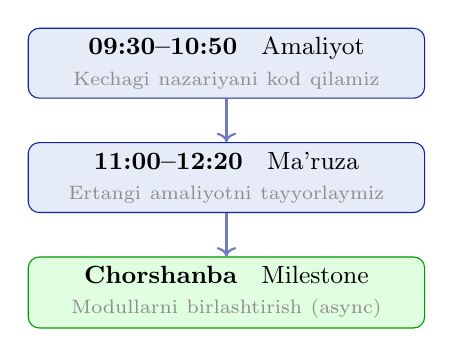
\begin{tikzpicture}[
        node distance=0.55cm,
        box/.style={rectangle,draw=cnublue,rounded corners=4pt,
                    fill=cnubluebg,text width=4.8cm,align=center,
                    minimum height=0.8cm,font=\small}
      ]
        \node[box] (am) {
          \textbf{09:30--10:50} \; Amaliyot\\
          \scriptsize\color{halfgray} Kechagi nazariyani kod qilamiz
        };
        \node[box,below=of am] (lec) {
          \textbf{11:00--12:20} \; Ma'ruza\\
          \scriptsize\color{halfgray} Ertangi amaliyotni tayyorlaymiz
        };
        \node[box,below=of lec,fill=green!12,draw=green!60!black] (ms) {
          \textbf{Chorshanba} \; Milestone\\
          \scriptsize\color{halfgray} Modullarni birlashtirish (async)
        };
        \draw[->,thick,cnublue!60] (am)--(lec);
        \draw[->,thick,cnublue!60] (lec)--(ms);
      \end{tikzpicture}
      \end{center}
    \end{column}
    \begin{column}{0.44\textwidth}
      \begin{tcolorbox}[defbox,title=Muhim qoida]
        \small \textbf{Ma'ruza $\to$ Amaliyot}:\\
        Har kuni 11:00 da eshitgan narsangizni \textbf{ertasi kuni} 09:30 da
        kodasizga aylantirасиз.\\[4pt]
        \textit{Shuning uchun ma'ruzani e'tibor bilan tinglash muhim!}
      \end{tcolorbox}
      \vspace{0.3em}
      \begin{tcolorbox}[warnbox]
        \small \textbf{Dars kunlari:}\\
        Dushanba, Seshanba,\\
        Payshanba, Juma.\\[2pt]
        16 kun $\times$ 4 soat = \textbf{64 soat}
      \end{tcolorbox}
    \end{column}
  \end{columns}
\end{frame}

% ================================================================
\section[4 hafta]{4 Haftalik Yo'l Xaritasi}
% ================================================================

\begin{frame}{4 Haftalik Mavzular}
  \begin{center}
  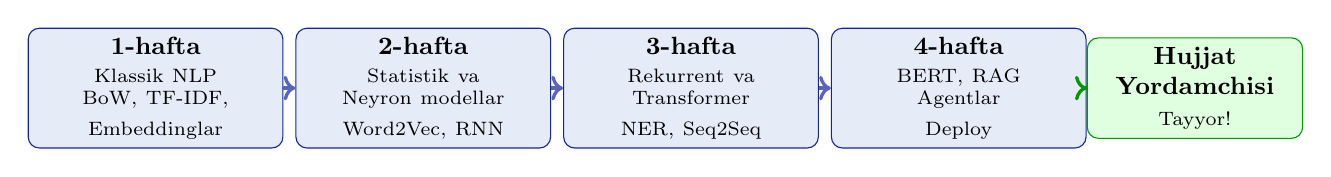
\begin{tikzpicture}[
    node distance=0.3cm and 0.25cm,
    wk/.style={rectangle,draw=cnublue,rounded corners=4pt,
               fill=cnubluebg,text width=3.0cm,align=center,
               minimum height=1.5cm,font=\small},
    goal/.style={rectangle,draw=green!60!black,rounded corners=4pt,
                 fill=green!12,text width=2.5cm,align=center,
                 minimum height=1.2cm,font=\small}
  ]
    \node[wk] (w1) at (0,0) {
      \textbf{1-hafta}\\[2pt]
      \scriptsize Klassik NLP\\
      \scriptsize BoW, TF-IDF,\\
      \scriptsize Embeddinglar
    };
    \node[wk] (w2) at (3.4,0) {
      \textbf{2-hafta}\\[2pt]
      \scriptsize Statistik va\\
      \scriptsize Neyron modellar\\
      \scriptsize Word2Vec, RNN
    };
    \node[wk] (w3) at (6.8,0) {
      \textbf{3-hafta}\\[2pt]
      \scriptsize Rekurrent va\\
      \scriptsize Transformer\\
      \scriptsize NER, Seq2Seq
    };
    \node[wk] (w4) at (10.2,0) {
      \textbf{4-hafta}\\[2pt]
      \scriptsize BERT, RAG\\
      \scriptsize Agentlar\\
      \scriptsize Deploy
    };
    \node[goal] (fin) at (13.2,0) {
      \textbf{Hujjat}\\
      \textbf{Yordamchisi}\\
      \scriptsize Tayyor!
    };
    \draw[->,very thick,cnublue!70] (w1)--(w2);
    \draw[->,very thick,cnublue!70] (w2)--(w3);
    \draw[->,very thick,cnublue!70] (w3)--(w4);
    \draw[->,very thick,green!60!black] (w4)--(fin);
  \end{tikzpicture}
  \end{center}
  \vspace{0.3em}
  \small
  \begin{tabular}{lll}
    \toprule
    \textbf{Hafta} & \textbf{Sanalar} & \textbf{Milestone} \\
    \midrule
    1 & 15--19 iyun & Preprocessing pipeline \\
    2 & 22--26 iyun & Klassik + neyron pipeline \\
    3 & 29 iyun -- 3 iyul & Neyron arxitekturalar \\
    4 & 6--10 iyul & Deploy + mudofaa \\
    \bottomrule
  \end{tabular}
\end{frame}

% ================================================================
\section[Kapstone]{Kapstone Loyiha: Modul Zanjiri}
% ================================================================

% ----------------------------------------------------------------
% [Q] KAPSTONE PIPELINE — TikZ
% ----------------------------------------------------------------
\begin{frame}{Kapstone: Siz Quradigan Tizim}
  \begin{center}
  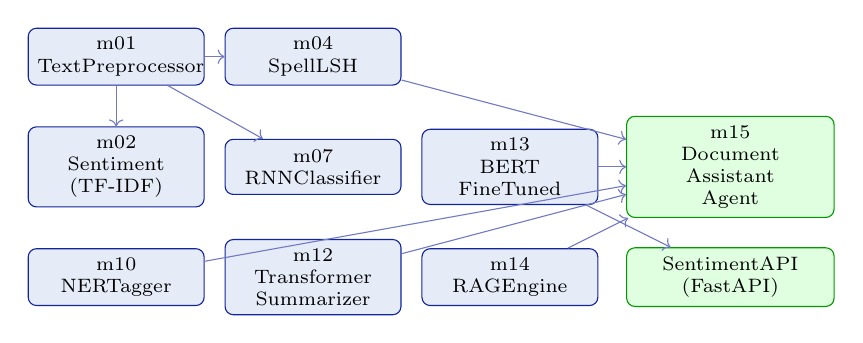
\begin{tikzpicture}[
    node distance=0.25cm and 0.05cm,
    mod/.style={rectangle,draw=cnublue,rounded corners=3pt,
                fill=cnubluebg,text width=2.0cm,align=center,
                minimum height=0.7cm,font=\scriptsize},
    final/.style={rectangle,draw=green!60!black,rounded corners=3pt,
                  fill=green!12,text width=2.4cm,align=center,
                  minimum height=0.7cm,font=\scriptsize}
  ]
    % Row 1: input + preprocessing
    \node[mod] (m01) at (0,0)    {m01\\TextPreprocessor};
    \node[mod] (m04) at (2.5,0)  {m04\\SpellLSH};
    % Row 2: classifiers
    \node[mod] (m02) at (0,-1.4) {m02\\Sentiment\\(TF-IDF)};
    \node[mod] (m07) at (2.5,-1.4){m07\\RNNClassifier};
    \node[mod] (m13) at (5.0,-1.4){m13\\BERT\\FineTuned};
    % Row 3: knowledge
    \node[mod] (m10) at (0,-2.8) {m10\\NERTagger};
    \node[mod] (m12) at (2.5,-2.8){m12\\Transformer\\Summarizer};
    \node[mod] (m14) at (5.0,-2.8){m14\\RAGEngine};
    % Agent
    \node[final] (m15) at (7.8,-1.4){m15\\Document\\Assistant\\Agent};
    % FastAPI
    \node[final] (api) at (7.8,-2.8){SentimentAPI\\(FastAPI)};

    % Arrows
    \draw[->,cnublue!60] (m01)--(m04);
    \draw[->,cnublue!60] (m01)--(m02);
    \draw[->,cnublue!60] (m01)--(m07);
    \draw[->,cnublue!60] (m13)--(m15);
    \draw[->,cnublue!60] (m14)--(m15);
    \draw[->,cnublue!60] (m12)--(m15);
    \draw[->,cnublue!60] (m04)--(m15);
    \draw[->,cnublue!60] (m10)--(m15);
    \draw[->,cnublue!60] (m13)--(api);
  \end{tikzpicture}
  \end{center}
  \vspace{0.2em}
  \begin{tcolorbox}[okbox]
    \small Har bir amaliyot \textbf{bir modul} (m01--m15) qo'shadi.
    Milestone da modullar birlashtiriladi. 16-kunda --- \textbf{mudofaa}.
  \end{tcolorbox}
\end{frame}

\begin{frame}{Kapstone: Har Kun Nima Quramiz?}
  \begin{center}
  \small
  \begin{tabular}{cll}
    \toprule
    \textbf{Kun} & \textbf{Modul} & \textbf{Nima qiladi?} \\
    \midrule
    2  & m01 TextPreprocessor   & Tokenizatsiya, stemming \\
    3  & m02 SentimentClassifier& TF-IDF + LogReg/NB \\
    4  & m03 PretrainedEmbedder & Word2Vec/.kv yuklash \\
    5  & m04 SpellLSHRetriever  & Imlo tuzatish + qidiruv \\
    6  & m05 Autocomplete       & N-gram to'ldirish \\
    7  & m06 CustomWord2Vec     & O'zbek embeddingleri \\
    8  & m07 RNNClassifier      & SimpleRNN tasniflash \\
    9  & m08 GRULSTMClassifier  & GRU vs LSTM \\
    11 & m10 NERTagger          & Bi-LSTM NER \\
    13 & m12 Summarizer         & Mini Transformer \\
    14 & m13 BERTClassifier     & BERT fine-tuning \\
    15 & m14 RAGEngine          & FAISS + LLM \\
    16 & m15 AgentLangChain     & ReAct agent \\
    M4 & SentimentAPI           & FastAPI deployment \\
    \bottomrule
  \end{tabular}
  \end{center}
\end{frame}

% ================================================================
\section[Hisoblash]{Hisoblash Resurslari}
% ================================================================

\begin{frame}{Kaggle Bepul GPU --- Qoidalar}
  \begin{columns}
    \begin{column}{0.50\textwidth}
      \begin{tcolorbox}[defbox,title=Resurslar]
        \small
        \textbf{GPU:} NVIDIA T4 yoki P100\\
        \textbf{VRAM:} 16 GB\\
        \textbf{Kvota:} $\approx$30 soat/hafta\\[4pt]
        \textbf{1--2-hafta:} CPU da ishlaymiz\\
        \textbf{3--4-hafta:} GPU kerak bo'ladi
      \end{tcolorbox}
      \vspace{0.4em}
      \begin{tcolorbox}[okbox,title=Tejash qoidasi]
        \small GPU ni faqat GPU belgili kunlarda yoqing.\\
        Sessiya tugaganda: \textbf{Accelerator $\to$ None}.
      \end{tcolorbox}
    \end{column}
    \begin{column}{0.46\textwidth}
      \begin{tcolorbox}[warnbox,title=Kvota tugasa nima bo'ladi?]
        \small GPU kvotangiz tugab qolsa --- haftalik
        yangilanishini kutasiz (dushanba). Shuning uchun:
        \begin{itemize}\setlength\itemsep{2pt}
          \item CPU ishini GPU da qilmang
          \item Notebook ni GPU da ochiq qoldirmang
          \item Checkpoint ni tez-tez saqlang
        \end{itemize}
      \end{tcolorbox}
      \vspace{0.3em}
      \begin{tcolorbox}[defbox,title=Dataset chegarasi]
        \small Har amaliyot dataset: $\leq 500$ MB\\
        FAISS indeks: $\leq 100$ MB
      \end{tcolorbox}
    \end{column}
  \end{columns}
\end{frame}

% ================================================================
\section[Ertaga]{Ertaga: Nima Tayyorlayman?}
% ================================================================

% ----------------------------------------------------------------
% [Q] BRIDGE — ertangi amaliyotga tayyorgarlik
% ----------------------------------------------------------------
\begin{frame}{Ertaga (2-Kun) Amaliyotga Tayyorgarlik}
  \begin{columns}
    \begin{column}{0.52\textwidth}
      \textbf{Ertangi amaliyot (09:30):}\\[4pt]
      \begin{tcolorbox}[defbox,title=P1 --- TextPreprocessor]
        \small
        O'zbek matni uchun tokenizatsiya,\\
        stopword filtrlash, stemming va\\
        BoW / TF-IDF vektorlash pipeline.\\[4pt]
        Moduli: \texttt{m01\_text\_preprocessor.py}
      \end{tcolorbox}
    \end{column}
    \begin{column}{0.44\textwidth}
      \textbf{Hozir bajaring:}
      \begin{enumerate}\setlength\itemsep{4pt}
        \item \texttt{d01\_orientatsiya.ipynb} ni to'liq ishga tushiring ---
              barcha tekshiruvlar \textbf{✓} bo'lishi kerak
        \item \texttt{capstone/contracts.py} ni o'qing ---
              \texttt{TextPreprocessor} imzosini toping
        \item \texttt{HISOB\_YARATISH.md} bo'yicha barcha hisoblarni oching
        \item Bugungi 11:00 ma'ruzasini e'tibor bilan tinglang:
              NLP asoslari va TF-IDF --- ertangi assertlarda kerak bo'ladi!
      \end{enumerate}
    \end{column}
  \end{columns}
\end{frame}

% ================================================================
\section[Manbalar]{Manbalar va Havolalar}
% ================================================================

% ----------------------------------------------------------------
% [R] MANBALAR
% ----------------------------------------------------------------
\begin{frame}{Asosiy Manbalar}
  \begin{columns}
    \begin{column}{0.48\textwidth}
      \textbf{Hisob yaratish:}
      \begin{itemize}\setlength\itemsep{3pt}
        \item \texttt{kaggle.com} --- notebook va dataset
        \item \texttt{huggingface.co} --- modellar va datasetlar
        \item \texttt{github.com} --- kapstone repo
      \end{itemize}
      \vspace{0.5em}
      \textbf{Kurs fayllari:}
      \begin{itemize}\setlength\itemsep{3pt}
        \item \texttt{capstone/SPEC.md} --- loyiha shartnomasi
        \item \texttt{capstone/contracts.py} --- modul imzolari
        \item \texttt{HISOB\_YARATISH.md} --- hisob sozlash yo'riqnomasi
        \item \texttt{LICENSES.md} --- datasetlar litsenziyasi
      \end{itemize}
    \end{column}
    \begin{column}{0.48\textwidth}
      \textbf{O'quv adabiyotlar:}
      \begin{itemize}\setlength\itemsep{3pt}
        \item Jurafsky \& Martin (2024). \textit{Speech and Language Processing}, 3rd ed. --- bepul PDF
        \item Goodfellow, Bengio, Courville (2016). \textit{Deep Learning} --- bepul onlayn
        \item fast.ai --- amaliy kurslar (bepul)
      \end{itemize}
      \vspace{0.5em}
      \begin{tcolorbox}[okbox]
        \small \textbf{Savol bo'lsa:}\\
        Dars davomida bevosita yoki\\
        kurs chat guruhida so'rang.
      \end{tcolorbox}
    \end{column}
  \end{columns}
\end{frame}

% ----------------------------------------------------------------
% Xulosa slayd
% ----------------------------------------------------------------
\begin{frame}{Bugun Nima Bajardik?}
  \begin{enumerate}\setlength\itemsep{8pt}
    \item \bajarildi Kursning maqsadi va 4-haftali yo'l xaritasini \textbf{ko'rdik}
    \item \bajarildi Har kunning tuzilmasini (ma'ruza $\to$ amaliyot) \textbf{tushundik}
    \item \bajarildi Kapstone loyiha modul zanjirini \textbf{ko'rib chiqdik}
    \item \bajarildi Kaggle GPU kvota qoidalarini \textbf{o'rgandik}
    \item \bajarildi Ertangi amaliyotga tayyorgarlik ro'yxatini \textbf{oldik}
  \end{enumerate}
  \vspace{0.5em}
  \begin{center}
    \begin{tcolorbox}[okbox,title=Keyingi qadam]
      \centering
      \textbf{11:00} --- 1-ma'ruza:\\
      NLP asoslari, TF-IDF va matnni qayta ishlash\\[4pt]
      \textit{(Ertangi amaliyot assertlari shu ma'ruzadagi sonlarga tayanadi)}
    \end{tcolorbox}
  \end{center}
\end{frame}

\end{document}
